%%%%% Copyright 2018 Nicholas J. Seewald

%%%%% This file is part of smart-figures

%%%%% smart-figures is free software: you can redistribute it and/or modify
%%%%% it under the terms of the GNU General Public License as published by
%%%%% the Free Software Foundation, either version 3 of the License, or
%%%%% (at your option) any later version.
%%%%% 
%%%%% This program is distributed in the hope that it will be useful,
%%%%% but WITHOUT ANY WARRANTY; without even the implied warranty of
%%%%% MERCHANTABILITY or FITNESS FOR A PARTICULAR PURPOSE.  See the
%%%%% GNU General Public License for more details.
%%%%% 
%%%%% You should have received a copy of the GNU General Public License
%%%%% along with this program.  If not, see <https://www.gnu.org/licenses/


\documentclass[border=3pt]{standalone}

\usepackage{tikz}
\usepackage[latin1]{inputenc}
\usetikzlibrary{positioning, arrows.meta, decorations.markings,calc}
\renewcommand{\familydefault}{\sfdefault}

\begin{document}
		
	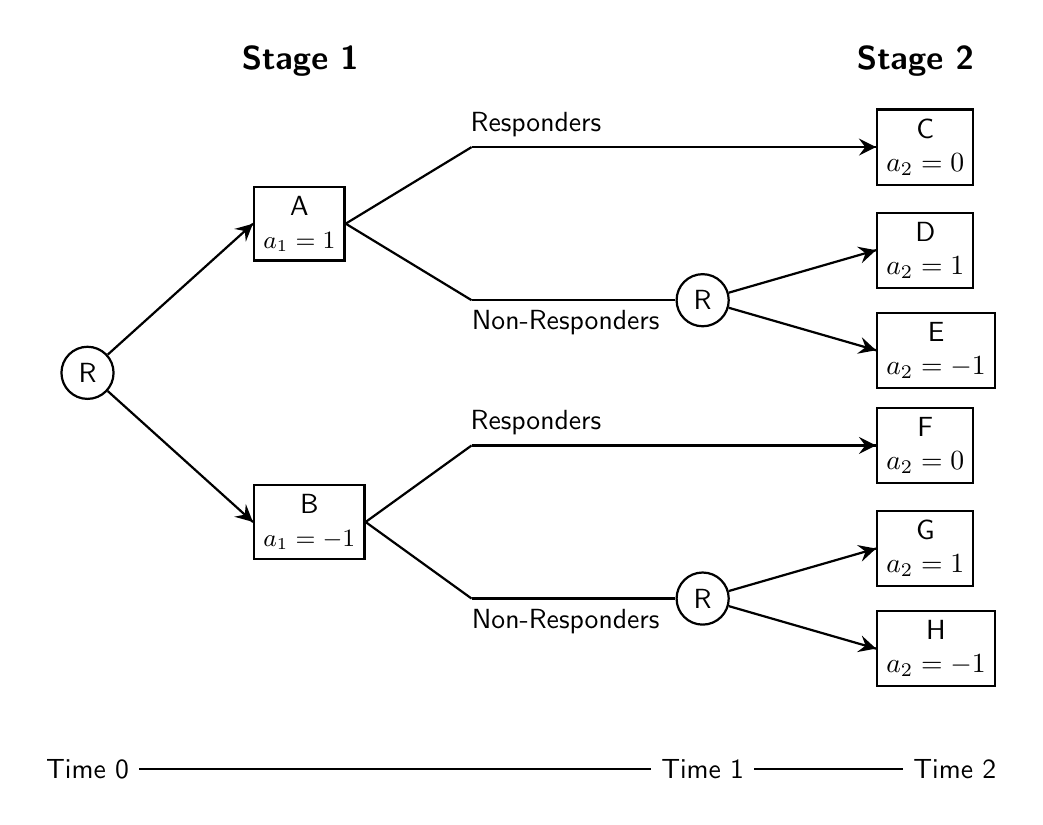
\begin{tikzpicture}[%
	%%%%%%%%%%%%%%%%%%%
	%%%%% STYLING %%%%%
	%%%%%%%%%%%%%%%%%%%
	%
	% NOTE: Do not leave blank uncommented lines here: compilation will fail
	%
	  %%% Styling for the randomization nodes (circled R)
		node distance=6mm,
		randomize/.style={
			circle, % shape of node
			minimum size=6mm, % size of node
			thick, % line width
			black, % line color
			draw
		},
		%
		%%% Additional styling applied to re-randomization nodes
		%%% (randomizations after the first one)
		rerand/.style={
			xshift = 15mm  % move the node 15mm to the 
		},
		%
		%%% Styling of treatment nodes
		treatment/.style={
			rectangle, % shape
			minimum size = 7mm, % size
			thick, % line weight
			black, % line color
			anchor=west, % place treatment at the right side of the column
			align=center, % text alignment
			draw
		},
		%
		%%% Styling for empty node used for placeholder to create "elbows" in 
		%%% path from first-stage treatment to second-stage treatment
		blank/.style={
			rectangle,
			minimum size=2mm
		},
		%
		%%% Styling for "subgroup" nodes at the end of the study identifying 
		%%% unique treatment paths (e.g., non-responders to A who received D in 
		%%% the second stage)
		subgroup/.style={
			rectangle, % shape
			rounded corners=1.5mm, % round corners of the rectangle to differentiate from treatment
			thin, % line weight
			minimum size=6mm, % size
			black, % line color
			draw
		},
		% 
		% Styling for the "Responders" arrow label
		rlabel/.style={
%			font=\footnotesize, % font size
			above, % place label above the arrow
			xshift=1mm, % move the label 1mm to the right (to match elbow)
			align=center % center the label in its column
		},
		% 
		% Styling for the "Non-Responders" arrow label
		nrlabel/.style={
%			font=\footnotesize, % font size
			below, % place label below the arrow
			xshift=-1mm, % move the label 1mm left to avoid clash with second-stage randomization
			align=left % align the label left in its column
		},
		%
		% Styling for arrows within the trial (i.e., from randomization to 
		% treatment, treatment to treatment, treatment to randomization)
		trialarrow/.style={
			thick, % line weight
			decoration={markings,mark=at position 1 with  {\arrow[scale=1.5,>=stealth]{>}}}, % arrow styling 
			% "stealth" indicates style of arrow
			% "scale" refers to relative size of arrowhead
			postaction={decorate} % create arrow
		},
		%
		% Styling from arrow going from second-stage treatment to subgroup node
		subsetarrow/.style={
			thin, % line width
			decoration={markings,mark=at position 1 with {\arrow[scale=1.2,>=stealth]{>}}}, % arrow styling
			% "stealth" indicates style of arrow
			% "scale" refers to relative size of arrowhead
			postaction={decorate} % create arrow
		}, thick
	]
				
	
	%% The nodes (randomizations, treatments, and subgroups, if applicable) are laid out in a TikZ matrix, which uses similar syntax as a usual LaTeX matrix. Ampersands (&) separate columns, and \\ separates lines.
	
	%% Nodes are created with \node [options] (name) {text}
	%% [options] references the styles created above as well as any 
	%% (name) allows for crossreferencing and connections
			
		\matrix[row sep=-2mm,column sep=12mm] { %
			%%% row sep changes separation between rows: -2mm keeps the figure relatively compact
			%%% column sep changes separation between columns: 12mm is generally the minimum needed to fit everything
			
			%%%% STAGE LABELS %%%%%
			&
			\node [align=center,xshift=6mm] (stage1) {\large \textbf{Stage 1}}; & & &
			\node [align=center,xshift=5mm] (stage2) {\large \textbf{Stage 2}};\\[5mm] %[5mm] adds space below this row (otherwise row sep takes over and the distance is too short)
			
			%%%%% TRIAL DESIGN %%%%%
			% Node designLabel can be used to provide a figure label (e.g., (a), (ii), etc.) if desired; otherwise, leave blank. Do not delete! This is used to compute placement of the first randomization node 	
			\node (designLabel) [blank] {}; 

			% blank nodes for alignment
			& &	\node (b1) [blank] {}; & \node (b2) [blank] {}; &
			
			% Treatment C: treatment for all responders to first-stage treatment A
			\node (C) [treatment] {C \\ $a_{2} = 0$};\\
			
			% Placeholder for first-stage treatment (this node is drawn and positioned below to ensure centering with respect to second-stage treatments)
			&  \node (stage1align) [treatment, white] {}; & & & \\
			& & & &
			
			% Treatment D: first of two possible second-stage treatments for non-responders to first-stage treatment A
			\node (D) [treatment] {D \\ $a_{2} = 1$};\\
			
			% blank node for alignment
			& &	\node (b3) [blank] {}; &
			
			% Second randomization for non-responders to first-stage treatment A
			% notice the application of the rerand style
			\node (R2) [randomize, rerand] {R}; & \\
			
			& & & & 

			% Treatment E: second of two possible second-stage treatments for non-responders to first-stage treatment A
			\node (E) [treatment] {E \\ $a_{2} = -1$};\\
			
			% Placeholder for first randomization (this node is drawn and positioned below to ensure centering with respect to second-stage treatments)
			\node [randomize,white] {};  & & & & \\
			
			% blank nodes for alignment
			& & \node (b4) [blank] {}; & \node (b5) [blank] {}; &
			
			% Treatment F: treatment for all responders to first-stage treatment B
			\node (F) [treatment] {F \\ $a_{2} = 0$};\\
			
			% blank node for alignment
			& \node [treatment, white] {}; & & & \\
			
			% Treatment G: first of two possible second-stage treatments for non-responders to first-stage treatment B
			& & & & \node (G) [treatment] {G \\ $a_{2} = 1$};\\
			& & \node (b6) [blank] {}; & \node (R3) [randomize, rerand] {R}; & \\
			
			% Treatment H: second of two possible second-stage treatments for non-responders to first-stage treatment B
			& & & & \node (H) [treatment] {H \\ $a_{2} = -1$};\\[1cm] %[1cm] adds space below H node for timeline
			
			%%%% TIMEPOINTS %%%%%
			
			\node (time0) [align=center, anchor=center] {Time 0};
			& & &
			% xshift=15mm aligns center of "Time 1" with center of second randomization
			\node (time1) [align=center, anchor=center, xshift=15mm] {Time 1};
			&
			% xshift=10mm aligns "Time 2" to right edge of second-stage treatment boxes
			\node (time2) [align=center, xshift = 10mm] {Time 2}; \\
		};
	
%		\draw[dashed,lightgray] (time1.north) -- (R2.south);
%		\draw[dashed,lightgray] (R2.north) -- (R3.south);
%		\draw[dashed,lightgray] (R3.north) --++(90:3.2cm);		
%		\draw[dashed,lightgray] (time2.north west) --++(90:33cm);
		
		%% Draw first-stage treatment A centered vertically between treatment C and the second randomization for non-responders to A
		\draw let \p1 = (stage1align.west), \p2=($(C) !.5! (R2)$) in node[treatment] at (\x1, \y2) (A) {A \\ \small{$a_{1} = 1$}};
		
		%% Draw first-stage treatment B centered vertically between treatment F and the second randomization for non-responders to B
		\draw let \p1 = (stage1align.west), \p2=($(F) !.5! (R3)$) in node[treatment] at (\x1, \y2) (B) {B \\ \small{$a_{1} = -1$}};
		
		%% Draw first randomization centered vertically between treatments A and B
		\draw let \p1 = (designLabel.north), \p2=($(A.north) !.5! (B.south)$) in node[randomize] at (\x1, \y2) (R1) {R};
		
%		\draw let \p3 = (stage1.north) \p4=($(C.north) !.5! (E.south)$) in node[treatment] at (\x3, \y4) (test) {A};
		
		%%%%%%%%%%%%%%%%%%%%%%
		%%%%% DRAW LINES %%%%%
		%%%%%%%%%%%%%%%%%%%%%%
		
		\draw[trialarrow] (R1) -- (A.west);
		\draw (A.east) -- (b1.center);
		\draw (A.east) -- (b3.center);
		\draw (b1.center) -- node [rlabel] {Responders} (b2.center);
		\draw (b3.center) -- node [nrlabel] {Non-Responders} (R2);
		\draw[trialarrow] (b2.center) -- (C);
		\draw[trialarrow] (R2) -- (D.west);
		\draw[trialarrow] (R2) -- (E.west);
		
		\draw[trialarrow] (R1) -- (B.west);
		\draw (B.east) -- (b4.center);
		\draw (B.east) -- (b6.center);
		\draw (b4.center) -- node [rlabel] {Responders} (b5.center);
		\draw[trialarrow] (b5.center) -- (F);
		\draw (b6.center) -- node [nrlabel] {Non-Responders} (R3);
		\draw[trialarrow] (R3) -- (G.west);
		\draw[trialarrow] (R3) -- (H.west);		
			
		% TIME LINES
		
		\draw (time0) -- (time1) -- (time2);
\end{tikzpicture}
\end{document}